\chapter{Guía de Uso}
\label{cap:descripcionTrabajo}
\label{cap:manualUsuario}

Este capítulo recoge los pasos que se deben seguir para poder utilizar la aplicación al completo.

\section{Dependencias de la aplicación}
\label{sec:dependeciasApp}
\subsection{Dependencias de Instalación}
	
	Para hacer uso de la aplicación, se requiere instalar herramientas de terceros. Estas dependencias se componen desde lenguajes de programación tales como Python, \textit{Node} y Reaper, hasta plugins e instrumentos. La lista de todas las dependencias se puede consultar en el Apéndice \ref{Appendix:Key1}.

    La aplicación funciona en los sistemas operativos \textit{Windows 10} y \textit{Windows 11}.

    Tras descargar los instrumentos y los presets, hay que proporcionarle a Reaper sendas rutas a los respectivos directorios.

    En \textit{Options > Preferences > Plug-ins > VSTs > VST pug-in paths} hay que añadir la ruta a los instrumentos que proporcionamos.

    En \textit{Options > Show Reaper resources path} se puede modificar la ruta al directorio de presets.

\subsection{Interfaz gráfica con \textit{TKInter}}
	\textit{TKInter} es la interfaz por defecto que \PythonLink{} ofrece a los desarrolladores para montar una 
    GUI (Interfaz Gráfica de Usuario por sus siglas en inglés).
	Esta herramienta viene integrada junto con Python, por lo que no requiere instalar ningún entorno ni herramienta adicional para hacer uso de ella.

\subsection{REAPER}
\label{subsec:manual-reaper}
	\href{https://www.reaper.fm/}{Reaper} es la DAW de producción musical que usamos en nuestra aplicación. Este entorno de edición y producción musical es el que nos permite renderizar el audio que generamos en nuestra aplicación. Es decir, nos permite agregar los instrumentos y efectos de audio que hacen sonar el MIDI generado o proporcionado por el usuario.
    
    Para el uso de la herramienta debemos instalar \textit{Reaper 7}, desde su \href{https://www.reaper.fm/download.php}{web oficial}. El usuario debe tener en cuenta que Reaper no es una DAW gratuita, pero permite un periodo de prueba con todas sus funcionalidades y donde podrá usar la herramienta sin ninguna limitación, tan sólo hay que esperar unos segundos y cerrar la pestaña que aparece explicando que estamos usando el periodo de prueba.


\section{Preparación del entorno}
\label{sec:app:preparacionEntorno}
Una vez instaladas las dependencias, se requiere una preparación del entorno de trabajo para poder ejecutar la aplicación.

\subsection{Entorno virtual}
Para poder ejecutar la app en un entorno virtual de Python, asegúrese de que la ejecución de scripts está activada en su plataforma Windows. 

La ejecución de scripts se puede activar desde un CMD con:
\textit{Set-ExecutionPolicy -Scope Process -ExecutionPolicy Bypass}.
Se puede desactivar con:
\textit{Set-ExecutionPolicy -Scope Process -ExecutionPolicy Default}.

Desde un CMD, en la raíz del repositorio, ejecute \textit{python -m venv env} para crear un entorno de python, depués \textit{./env/Scripts/activate} para activar el entorno virtual. Crear el entorno solo es necesario hacerlo una vez, pero será necesario activarlo cada vez que se abra un CMD, ya que por defecto está desactivado. Con el entorno activado, puede ejecutar el comando \textit{pip intall -r requirements.txt} para instalar todas las dependencias de la aplicación automáticamente.

\subsection{Ejecución de scripts con Reaper}
Por defecto, Reaper solo permite la ejecución de scripts de Lua y de EEL (\textit{Embedded Extensible Language}).

Para que nuestra aplicación se pueda comunicar con Reaper, es necesario tener activada la opción \textit{permitir ejecución de scripts de Python}. Dentro de Reaper, debemos seleccionar el apartado \textit{Opciones > Preferencias} (o atajo de teclado\textit{ Ctrl+P}) y buscar el apartado \textit{ReaScript} dentro del apartado \textit{Plug-ins}. Una vez en esta pestaña, marcaremos la casilla \textit{Enable Python for use with ReaScript} y le proporcionaremos la ruta a nuestro ejecutabl de Python 3.9.0 (Apéndice \ref{Appendix:Key1}), así como el nombre de la \textit{.dll} de Python (\textit{python39.dll} en el caso de usar la versión que recomendamos) Pulsamos \textit{apply} y debería indicarnos que Python está instalado correctamente, reiniciamos Reaper y estamos listos para usar la herramienta.

\section{Generación de audio}
\label{sec:app:generacionAudio}
	Esta es la primera pestaña de \appName{}, la que aparecerá nada más abrir la aplicación (Figura \ref{fig:generationTab}).

\begin{figure}[h]
    \begin{center}
        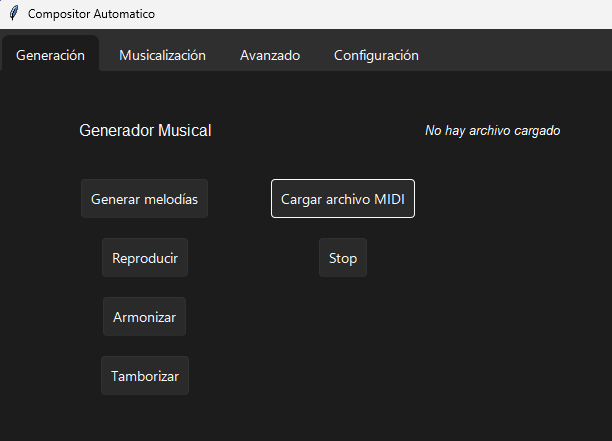
\includegraphics[scale=0.75]{Imagenes/Bitmap/generationTab.png}
    \end{center}
    \caption{Pestaña \textit{\generationTabName{}}}
    \label{fig:generationTab}
\end{figure}

Esta pestaña reúne las funcionalidades que permiten al usuario generar MIDI. Estas funcionalidades se dividen en Generar melodía, Reproducir, Armonizar y Tamborizar.

\begin{itemize}
  \item Generar: Genera MIDI de acuerdo con el generador activo. Para cambiar el generador de midi, ver la Sección \ref{subsec:app:alternarGenerador}.
  \item Cargar archivo MIDI: Carga un archivo .mid desde el sistema de ficheros del usuario.
  \item Reproducir: Reproduce la melodía generada a modo prueba con un sintetizador simple.
  \item Armonizar: Armoniza la melodía generada. Ver la Sección \ref{sec:arm:armonia} para más detalle.
  \item Tamborizar: Genera el MIDI asociado a la percusión. La sección \ref{subsec:generacion-percusion-propia} contiene más información acerca de cómo se genera la percusión.
\end{itemize}

\section{Selección de Temática y Sonorización}
\label{sec:SeleccionTematica}

Esta sección describe la pestaña \tematicTabName{} de la aplicación (Figura \ref{fig:tematicTab}). 

\begin{figure}[h]
    \begin{center}
        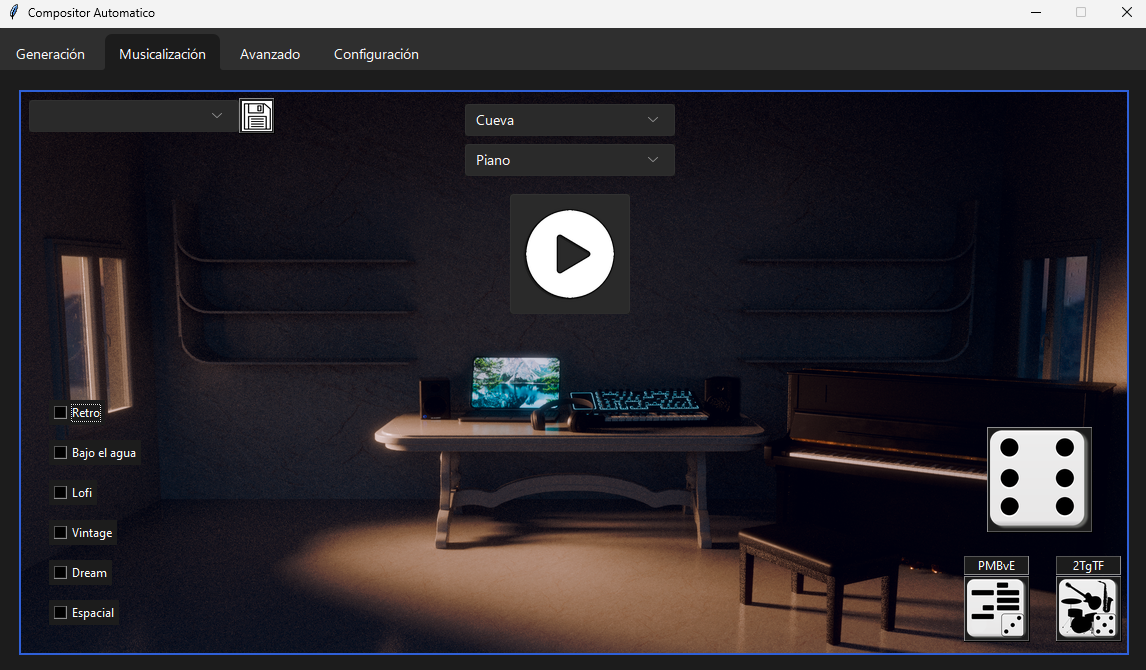
\includegraphics[scale=0.45]{Imagenes/Bitmap/tematicTab.png}
    \end{center}
    \caption{Pestaña \tematicTabName{}}
    \label{fig:tematicTab}
\end{figure}

En esta pestaña disponemos de varias opciones para dirigir la sonorización del MIDI generado en la pestaña \nameref{sec:app:generacionAudio}.

\subsection{Temáticas}
\label{subsec:app:themes}

Las temáticas afectan a la instrumentación del arreglo musical. En la parte superior de la Figura \ref{fig:tematicTab}, encontramos un desplegable con las posibles temáticas que se pueden seleccionar. Por defecto viene con la temática Pradera. El estilo del fondo irá cambiando según la temática seleccionada, reflejando la configuración activa. 
Las temáticas disponibles son las siguientes:

\begin{itemize}
    \item \textbf{Pradera}: Sonidos de guitarra, piano y cuerdas. Genera la sensación de estar al aire libre en una pradera o un bosque. En ocasiones puede llegar a sonar a Aventura.
    \item \textbf{Piano}: Un único piano interpretará todo el arreglo.
    \item \textbf{Desierto}: Sitars, flautas, guitarras y percusiones que dan la sensación de estar en un desierto.
    \item \textbf{Nieve}: Sonidos brillantes, ukeleles y kalimbas que nos sitúan en un paisaje nevado.
    \item \textbf{Pirata}: Guitarras, percusiones, acordeones y violines que bien podría llevar un pirata en su barco. 
    \item \textbf{Selva}: Marimbas y una gran variedad de sonidos de percusión sonando simultáneamente interpretando los ritmos de la selva.
    \item \textbf{Épico}: Una orquesta entera interpretando el arreglo. 
    \item \textbf{Tenebroso}: Sonidos lúgubres con timbres no muy agradables que generan tensión constante.
    \item \textbf{Agua}: Sonidos suaves y burbujeantes generan la sensación de estar flotando.
    \item \textbf{Asiático}: Instrumentos tradicionales asiáticos mezclados con sonidos modernos.
    \item \textbf{Rock}: Guitarras eléctricas con mucha distorsión.
    \item \textbf{Pop}: Sonidos modernos presentes en la música pop actual.
    \item \textbf{Tecno}: Percusión de música disco y varios sintetizadores sonando a la vez.
\end{itemize}

\subsection{Entorno}
\label{subsec:app:reverb}
Justo encima del desplegable de temáticas encontramos el desplegable de entornos. Este desplegable nos dará la opción de elegir dónde se simulará que suena nuestra canción, es decir, cambiará la reverberación que se aplicará a la mezcla.

\subsection{Efectos}
\label{subsec:app:effects}

En la parte inferior izquierda se encuentran varias \textit{checkboxes} asociadas a efectos que se pueden aplicar a la canción. Los cambios en estos modificadores también se ven reflejados en el estilo del fondo de esta pestaña de la aplicación.

Los efectos disponibles son los siguientes:

\begin{itemize}
    \item \textbf{Retro}: Disminuye la tasa de bits y la frecuencia de muestreo, reduciendo la calidad del sonido. Esto hace que la mezcla suene como lo haría en una consola antigua.
    \item \textbf{Bajo el agua}: Ralentiza todos los sonidos para generar la sensación de estar buceando.
    \item \textbf{Lofi}: Agrega un filtro Lofi de entre varios posibles. Esto conlleva la disminución de la calidad del sonido, el filtrado de frecuencias agudas, la adición de ruido de fondo (como el ruido de una cinta antigua) y algunas imperfecciones en el tono del sonido.
    \item \textbf{Vintage}: Saturación analógica y pedales de reverberación de agregará la calidez característica de una grabación en cinta antigua.
    \item \textbf{Dream}: Ralentiza los sonidos y los desafina ligeramente para generar una sensación psicodélica.
    \item \textbf{Espacial}: Coloca todos los sonidos en el espacio. Ideal para temas espaciales o de música \textit{ambient}.
\end{itemize}



\subsection{Semillas}
\label{subsec:app:seed}
En la parte inferior derecha de la Figura \ref{fig:tematicTab} se encuentra un botón con forma de dado, mostrando un seis. Este dado aleatoriza las semillas de instrumentos y de arreglos. Estas semillas serán las que se utilicen para sonorizar el MIDI una vez se pulse el botón de reproducir que hay en medio de la pantalla. Una misma semilla generará los mismos instrumentos y pistas siempre que la configuración de \nameref{subsec:app:themes} sea la misma. Es decir, para dos casos de uso donde la semilla sea la misma pero la temática o los modificadores (\textit{checkboxes}) sean distintos, la generación final de instrumentos y pistas será distinta.

La semilla de instrumentos es la que está encima del botón de dado que muestra un 5, junto a varios instrumentos (Figura \ref{fig:tematicTab}). Esta semilla cambia la asignación de instrumentos sin modificar el MIDI de las pistas. Esta semilla se puede cambiar por ejemplo si se desea modificar los instrumentos sin afectar al arreglo o distribución de los ítems MIDI.

La semilla de arreglos es la que se sitúa encima del botón de dado que muestra un 3, junto a unas barras horizontales negras \ref{fig:tematicTab}. Esta semilla cambia la disposición del MIDI generado en las distintas pistas de Reaper. Esta semilla se puede cambiar por ejemplo si se desea modificar el arreglo sin afectar a la asignación de instrumentos.

Cada semilla se puede cambiar mediante su botón asociado. También se puede introducir una semilla a mano directamente escribiendo sobre la entrada de texto de la semilla.


\subsection{Presets}
\label{subsec:app:presets}
Los presets son configuraciones de la pestaña \tematicTabName{} que se guardan dentro de la aplicación. Estas configuraciones albergan el estado de la temática, las \textit{checkboxes} y la semilla seleccionadas al momento de haberlas guardado. La configuración actual de la pestaña \tematicTabName{} se puede guardar haciendo \textit{click} en el botón que tiene el icono de la Figura \ref{fig:savePresetIcon}.

\begin{figure}[h]
    \begin{center}
        
\includegraphics[scale=0.25]{Imagenes/Bitmap/saveIcon.png}
    \end{center}
    \caption{Icono de guardado}
    \label{fig:savePresetIcon}
\end{figure}

Al pulsar este botón, se abrirá una ventana solicitando un nombre para el preset (Figura \ref{fig:savePresetIcon}). Para crear un nuevo preset, basta con escribir un nombre de preset que no esté registrado ya. Si se introduce un nombre de preset ya registrado, este se sobrescribirá con la información del nuevo estado de la pestaña \tematicTabName{}.

Para recuperar un preset, basta con utilizar el desplegable situado en la parte superior izquierda de la pestaña y seleccionar el nombre del preset. Esto actualizará la información de la pestaña con la que había en el momento en el que se guardó ese preset, es decir: temática, \textit{checkboxes} y semilla.

\section{Renderizado: Descarga de los resultados}
Al pulsar el botón de \textit{Play}, se abrirá REPER automáticamente, disponiendo las pistas con el MIDI y los instrumentos generados en los pasos previos de la aplicación.

A partir de este punto el usuario tiene total libertad de trabajar con Reaper de forma autónoma, con la propia interfaz de Reaper. Para renderizar y guardar el resultado, en \textit{File > Render} se puede seleccionar el formato de compresión, el nombre de archivo y la ruta de guardado, así como otras características propias de Reaper.

\section{Modo avanzado}
\label{sec:app:advancedMode}
El objetivo principal de la aplicación es ofrecer a los usuarios una forma sencilla de generar temas musicales. No obstante, está incluida la posibilidad de relizar acciones avanzadas para los usuarios más avezados de la aplicación, así como los que cuentan con conicimiento musical previo.

La posibilidad de editar en REAPER los temas musicales generados por nuestra aplicación sigue existiendo, tal y como está planteado en la sección anterior, al pulsar el botón de \textit{Play}. Esto permite al usuario poder trabajar directamente en Reaper en lugar de centrarse en nuestra aplicación, a partir de los MIDIs e instrumentos generados por \appName{}

En los apartados siguientes veremos las acciones posibles dentro de la pestaña \advancedTabName{} de la aplicación (Figura \ref{fig:advancedTab})

\begin{figure}[h]
    \begin{center}
        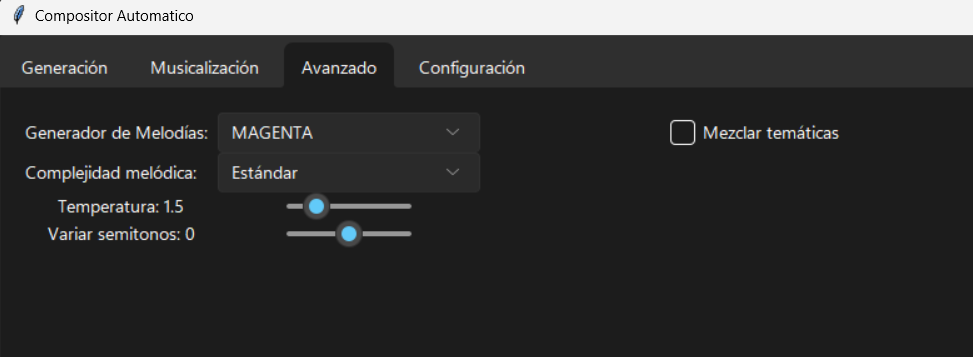
\includegraphics[scale=0.7]{Imagenes/Bitmap/advancedTab.png}
    \end{center}
    \caption{Pestaña avanzada}
    \label{fig:advancedTab}
\end{figure}

\subsection{Alternar Generador}
\label{subsec:app:alternarGenerador}
Esta opción permite cambiar el modo de generación de la melodía en la pestaña \generationTabName{}. Los generadores disponibles son Cadenas de Markov, Redes Neuronales Recurrentes y Magenta. Ver la Sección \ref{cap:generacionMusical} para más información acerca de los modos de generación musical. 

\subsection{Temperatura}
\label{subsec:app:temperature}
La temperatura influye en cómo el generador produce el MIDI para las melodías. Un valor bajo hace que el generador tome decisiones menos arriesgadas, con melodías más simples, mientras que valores altos dotan de un carácter experimental al generador. Por defecto, como muestra la Figura \ref{fig:advancedTab}, el valor de temperatura se encuentra a 1'5.

\subsection{Mezclar temáticas}
\label{subsec:app:mixThemes}

La opción mezclar temáticas permite asignar a cada pista de Reaper una temática distinta, en lugar de aplicar la misma temática a todas.

\begin{figure}[h]
    \begin{center}
        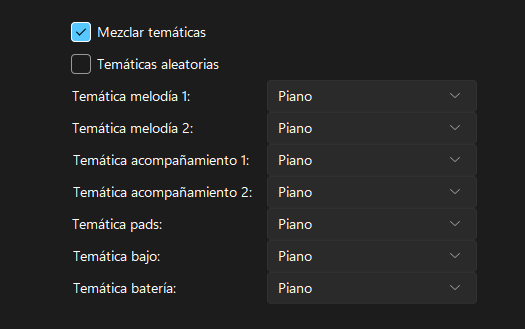
\includegraphics[scale=0.7]{Imagenes/Bitmap/mixedThemes.png}
    \end{center}
    \caption{Mezclar temáticas}
    \label{fig:mixThemes}
\end{figure}

En la Figura \ref{fig:mixThemes} se puede observar qué pista se asociará con qué temática. Por defecto, cuando la opción temáticas aleatorias está desactivada, se aplicarán a todas las pistas la temática seleccionada en la pestaña \tematicTabName{}. De este modo, el usuario puede ir modificando la temática de cada pista a partir de una temática raíz.

Las temáticas añadidas al desplegable se incluirán en el preset al momento de guardarlo, pudiendo ser recuperado, como se indica en la sección \nameref{subsec:app:presets}. No obstante, solo se aplicará en la musicalización en Reaper si la opción Mezclar temáticas está activada.

La opción Temáticas aleatorias asigna una temática aleatoria a cada pista, como se refleja en la Figura \ref{fig:randomizeThemes}

\begin{figure}[h]
    \begin{center}
        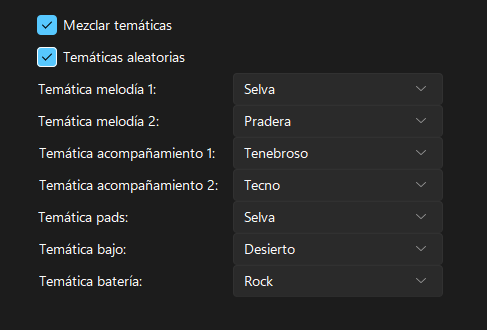
\includegraphics[scale=0.7]{Imagenes/Bitmap/randomThemes.png}
    \end{center}
    \caption{Aleatorización de temáticas}
    \label{fig:randomizeThemes}
\end{figure}


\subsection{Variar semitonos}
Varía la tonalidad de la canción el número de semitonos indicados en la Figura \ref{fig:advancedTab}. Esta variación se aplica a la señal MIDI que reciben los intrumentos virtuales que generan el sonido en Reaper. No modifica en modo alguno el sonido una vez generado, por tanto no se pierde calidad de la mezcla final por usar esta funcionalidad (como sucedería si se varía la tonalidad en el sonido ya generado).

\section{Configuración}
\label{sec:app:conFiguration}

La pestaña de configuración permite reorganizar los recursos de la aplicación.

\begin{itemize}
    \item Ruta de reaper: La ruta absoluta a reaper es utilizada por la aplicación para poder encontrar el ejecutable de reaper a la hora de reproducir el contenido generado por \appName{}. Por defecto, REAPER se busca en \textit{C:/Program Files/REAPER (x64)/reaper.exe}. Si su ruta absoluta a Reaper es distita a esta, es importante que actualice esta opción para poder usar la app correctamente.
\end{itemize}

\section{Ayuda y Tooltips}

Las Tooltips son descripciones de texto que muestran el efecto o función de un elemento. Esto incluye botones, entradas de texto, desplegables, etc. Para ver la Tooltip de una herramienta, sitúe el cursor encima de la herramienta.